\documentclass[aspectratio=169,11pt]{beamer}
\usetheme{Madrid}
\usecolortheme{seahorse}
\usepackage[utf8]{inputenc}
\usepackage[T1]{fontenc}
\usepackage{lmodern}
\usepackage{amsmath,amssymb,mathtools}
\usepackage{graphicx}
\usepackage{booktabs,array,multicol}
\usepackage{tikz}
\usetikzlibrary{positioning}
\graphicspath{{../../assets/}{./}}
\setbeamertemplate{navigation symbols}{}
\definecolor{iteraBlue}{RGB}{23,70,125}
\definecolor{iteraGold}{RGB}{175,145,55}
\definecolor{softBlue}{RGB}{235,241,250}
\definecolor{softGold}{RGB}{255,249,232}
\definecolor{iteraRed}{RGB}{170,35,35}
\setbeamercolor{title}{fg=iteraBlue}
\setbeamercolor{frametitle}{fg=iteraBlue,bg=softBlue}
\setbeamercolor{block title}{bg=iteraBlue,fg=white}
\setbeamercolor{block body}{bg=softBlue,fg=black}
\setbeamercolor{example title}{bg=iteraGold,fg=black}
\setbeamercolor{example body}{bg=softGold,fg=black}
\setbeamercolor{alertblock title}{bg=iteraRed,fg=white}
\setbeamercolor{alertblock body}{bg=red!5,fg=black}
\setbeamertemplate{blocks}[rounded][shadow=true]
\setbeamerfont{frametitle}{size=\large,series=\bfseries}
\setbeamerfont{footline}{size=\tiny}
\newcommand{\course}{Matematika 3 - KL25-21001}
\newcommand{\kelas}{Kelas RB}
\newcommand{\jadwal}{Kamis, 14.50--17.30 - E302}
\newcommand{\pengajar}{Rifky Fauzi}
\newcommand{\Lap}{\mathcal{L}}
\newcommand{\invLap}{\mathcal{L}^{-1}}
\newcommand{\Y}{Y(p)}
\newcommand{\F}{F(p)}
\newcommand{\dd}{\,\mathrm{d}}
\setbeamertemplate{footline}{%
\leavevmode\hbox{%
\begin{beamercolorbox}[wd=.40\paperwidth,ht=2.5ex,dp=1ex,leftskip=1em]{author in head/foot}\color{gray}\pengajar\end{beamercolorbox}%
\begin{beamercolorbox}[wd=.43\paperwidth,ht=2.5ex,dp=1ex,center]{title in head/foot}\color{gray}\course\end{beamercolorbox}%
\begin{beamercolorbox}[wd=.17\paperwidth,ht=2.5ex,dp=1ex,rightskip=1em plus1fil]{date in head/foot}\hfill\color{gray}\insertframenumber/\inserttotalframenumber\end{beamercolorbox}}}
\title[Transformasi Laplace]{Pertemuan 3\\Transformasi Laplace}
\subtitle{Dari definisi dan tabel sampai penyelesaian PDB}
\author{\pengajar}
\institute{Program Studi Teknik Kelautan\\Institut Teknologi Sumatera}
\date{\kelas\quad |\quad \jadwal}
\begin{document}

\begin{frame}
\titlepage\vspace{-0.45cm}\centering
\includegraphics[height=0.92cm]{itera_logo.png}
\end{frame}

\section{Peta Keterampilan}
\begin{frame}{Tujuan Pertemuan}
Setelah pembelajaran ini, mahasiswa dapat:
\begin{enumerate}
\item menjelaskan definisi dan kegunaan Transformasi Laplace;
\item menghitung transformasi dari \textbf{definisi integral};
\item memakai \textbf{tabel dan sifat linearitas} untuk bentuk eksponen, sinus, cosinus, dan gabungannya;
\item menghitung \textbf{transformasi balik} melalui tabel, pergeseran, dan pecahan parsial;
\item menyelesaikan \textbf{PDB beserta syarat awal} melalui aljabar di domain transformasi.
\end{enumerate}
\end{frame}

\begin{frame}{Alur Penyelesaian Soal}
\begin{center}
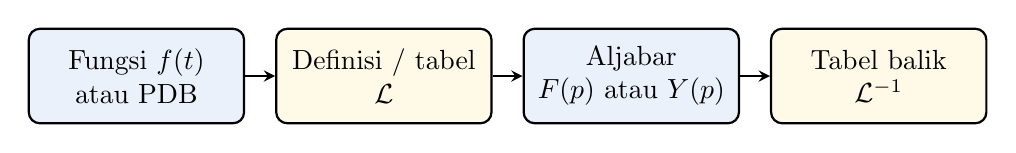
\begin{tikzpicture}[>=stealth,thick,node distance=0.38cm,every node/.style={align=center}]
\node[draw,rounded corners,fill=softBlue,text width=2.5cm,minimum height=1.2cm] (a) {Fungsi $f(t)$ \\ atau PDB};
\node[draw,rounded corners,fill=softGold,text width=2.5cm,minimum height=1.2cm,right=of a] (b) {Definisi / tabel\\ $\Lap$};
\node[draw,rounded corners,fill=softBlue,text width=2.5cm,minimum height=1.2cm,right=of b] (c) {Aljabar\\ $F(p)$ atau $Y(p)$};
\node[draw,rounded corners,fill=softGold,text width=2.5cm,minimum height=1.2cm,right=of c] (d) {Tabel balik\\ $\invLap$};
\draw[->] (a)--(b);\draw[->] (b)--(c);\draw[->] (c)--(d);
\end{tikzpicture}
\end{center}
\begin{block}{Jenis keterampilan yang akan dilatih}
\textbf{Transformasi langsung} $\to$ \textbf{transformasi balik} $\to$ \textbf{solusi PDB}.
\end{block}
\begin{alertblock}{Ingat}
Jika soal berisi $y(0)$ atau $y'(0)$, gunakan rumus transformasi \emph{turunan}; bukan hanya tabel fungsi dasar.
\end{alertblock}
\end{frame}

\section{Definisi dan Perhitungan Integral}
\begin{frame}{Definisi Transformasi Laplace}
\begin{block}{Dari fungsi semula ke fungsi transformasi}
\[
\boxed{F(p)=\Lap\{f(t)\}=\int_0^\infty e^{-pt}f(t)\dd t.}
\]
\end{block}
\begin{itemize}
\item $t$ adalah variabel pada fungsi asal; $p$ adalah variabel transformasi.
\item Integral \textbf{tak wajar}: hitung sebagai limit batas atas $R\to\infty$.
\item Nilai $p$ harus dipilih sehingga integral \textbf{konvergen}.
\item Boas memakai huruf $p$; penulisan dengan $s$ berarti hal yang sama.
\end{itemize}
\end{frame}

\begin{frame}{Bagaimana Fungsi Berubah Setelah Ditransformasi?}
\[
\boxed{f(t)=e^{-2t}}\quad\xrightarrow{\ \Lap\ }\quad
\boxed{F(p)=\frac{1}{p+2}.}
\]
\begin{columns}[T]
\column{.48\textwidth}
\begin{block}{Fungsi asal}
\centering
\begin{tikzpicture}[x=0.88cm,y=1.8cm]
\draw[->](0,0)--(4.6,0) node[right] {$t$};\draw[->](0,0)--(0,1.16);
\draw[thick,iteraBlue,domain=0:4.3,samples=70] plot (\x,{exp(-2*\x)});
\node[anchor=east,font=\scriptsize] at (0,1) {$1$};
\end{tikzpicture}
\end{block}
\column{.48\textwidth}
\begin{block}{Fungsi transformasi}
\centering
\begin{tikzpicture}[x=0.88cm,y=2.9cm]
\draw[->](0,0)--(4.6,0) node[right] {$p$};\draw[->](0,0)--(0,0.67);
\draw[thick,iteraGold,domain=0:4.3,samples=70] plot (\x,{1/(\x+2)});
\node[anchor=east,font=\scriptsize] at (0,.5) {$1/2$};
\end{tikzpicture}
\end{block}
\end{columns}
\vspace{3mm}\centering\scriptsize Fungsi awal berubah menjadi fungsi rasional dalam variabel $p$.
\end{frame}

\begin{frame}{Contoh 1: Konstanta dari Definisi}
Hitung $\Lap\{1\}$ dari integral, dengan $p>0$.
\begin{align*}
F(p)&=\lim_{R\to\infty}\int_0^R e^{-pt}\dd t\\
&=\lim_{R\to\infty}\left[-\frac{1}{p}e^{-pt}\right]_0^R\\
&=\lim_{R\to\infty}\frac{1-e^{-pR}}{p}
=\boxed{\frac{1}{p}}.
\end{align*}
\begin{alertblock}{Syarat konvergensi}
Untuk $p>0$, $e^{-pR}\to0$; karena itulah hasil ini berlaku.
\end{alertblock}
\end{frame}

\begin{frame}{Contoh 2: Fungsi Eksponen dari Definisi}
Hitung transformasi $f(t)=e^{at}$ untuk konstanta riil $a$.
\begin{align*}
\Lap\{e^{at}\}
&=\lim_{R\to\infty}\int_0^R e^{-pt}e^{at}\dd t\\
&=\lim_{R\to\infty}\int_0^R e^{-(p-a)t}\dd t\\
&=\lim_{R\to\infty}\frac{1-e^{-(p-a)R}}{p-a}\\
&=\boxed{\frac{1}{p-a}},\qquad p>a.
\end{align*}
\begin{exampleblock}{Baca tandanya}
$e^{+2t}\mapsto 1/(p-2)$, sedangkan $e^{-2t}\mapsto 1/(p+2)$.
\end{exampleblock}
\end{frame}

\begin{frame}{Contoh 3: Penurunan Intensitas}
Intensitas cahaya pada kedalaman $t$ memenuhi model $I(t)=I_0e^{-\mu t}$, $\mu>0$.
\[
\begin{aligned}
\Lap\{I(t)\}
&=I_0\int_0^\infty e^{-pt}e^{-\mu t}\dd t\\
&=I_0\int_0^\infty e^{-(p+\mu)t}\dd t\\
&=\boxed{\frac{I_0}{p+\mu}},\qquad p>-\mu.
\end{aligned}
\]
\begin{block}{Interpretasi}
Profil intensitas eksponensial dalam variabel kedalaman diubah menjadi fungsi rasional $p$. Variabel bebas tidak harus selalu waktu.
\end{block}
\end{frame}

\begin{frame}{Sinus dan Cosinus: Siapkan Dua Integral}
Untuk $p>0$ dan $b$ real, definisikan
\[
I=\int_0^\infty e^{-pt}\sin(bt)\dd t,
\qquad J=\int_0^\infty e^{-pt}\cos(bt)\dd t.
\]
Gunakan integral parsial pada \emph{keduanya}:
\begin{align*}
I&=\left[-\frac{e^{-pt}\sin(bt)}p\right]_0^\infty
 +\frac bp\int_0^\infty e^{-pt}\cos(bt)\dd t
 =\frac bp J,\\[1mm]
J&=\left[-\frac{e^{-pt}\cos(bt)}p\right]_0^\infty
 -\frac bp\int_0^\infty e^{-pt}\sin(bt)\dd t
 =\frac1p-\frac bp I.
\end{align*}
\end{frame}

\begin{frame}{Hasil Integral Sinus dan Cosinus}
Dari $I=\frac bpJ$ dan $J=\frac1p-\frac bpI$ diperoleh
\[
I=\frac bp\left(\frac1p-\frac bp I\right)
\quad\Longrightarrow\quad (p^2+b^2)I=b.
\]
\begin{block}{Dua hasil yang perlu dikenal}
\[
\boxed{\Lap\{\sin bt\}=\frac{b}{p^2+b^2}},\qquad
\boxed{\Lap\{\cos bt\}=\frac{p}{p^2+b^2}}.
\]
\end{block}
\small Untuk parameter $b$ real dan $p>0$. Perhatikan \textbf{pembilangnya berbeda}: sinus menghasilkan $b$, cosinus menghasilkan $p$.
\end{frame}

\begin{frame}{Contoh 4: Sinus dari Integral}
Hitung $\Lap\{\sin 3t\}$, tidak langsung membaca tabel.
\[
\begin{aligned}
I_3&=\int_0^\infty e^{-pt}\sin(3t)\dd t,\\
J_3&=\int_0^\infty e^{-pt}\cos(3t)\dd t,\\
I_3&=\frac3pJ_3,\qquad J_3=\frac1p-\frac3p I_3,\\
(p^2+9)I_3&=3.
\end{aligned}
\]
\[
\boxed{\Lap\{\sin 3t\}=\frac3{p^2+9}.}
\]
\end{frame}

\begin{frame}{Contoh 5: Cosinus dari Integral}
Hitung $\Lap\{\cos 2t\}$.
\[
\begin{aligned}
I_2&=\int_0^\infty e^{-pt}\sin(2t)\dd t,
\qquad J_2=\int_0^\infty e^{-pt}\cos(2t)\dd t,\\
I_2&=\frac2pJ_2,\qquad J_2=\frac1p-\frac2pI_2,\\
J_2&=\frac1p-\frac4{p^2}J_2.
\end{aligned}
\]
\[
\boxed{\Lap\{\cos2t\}=J_2=\frac{p}{p^2+4}.}
\]
\end{frame}

\begin{frame}{Contoh 6: Sudut dengan Parameter Konstan}
Diberikan $f(t)=0.4\sin(kx-t)$; $k$ dan $x$ \textbf{konstan}.
\[
\sin(kx-t)=\sin(kx)\cos t-\cos(kx)\sin t.
\]
Dengan linearitas,
\[
\begin{aligned}
\Lap\{f(t)\}
&=0.4\left(\sin(kx)\frac{p}{p^2+1}
-\cos(kx)\frac1{p^2+1}\right)\\
&=\boxed{\frac{0.4[p\sin(kx)-\cos(kx)]}{p^2+1}}.
\end{aligned}
\]
\begin{alertblock}{Perhatikan variabel integral}
Transformasi dilakukan terhadap $t$, bukan terhadap $x$.
\end{alertblock}
\end{frame}

\begin{frame}{Linearitas: Menggabungkan Hasil}
Dari sifat linear integral,
\[
\boxed{\Lap\{af(t)+bg(t)\}=aF(p)+bG(p)}.
\]
\begin{exampleblock}{Contoh}
\[
\begin{aligned}
\Lap\{3e^{-2t}-2\sin3t+\cos2t\}
&=\frac3{p+2}-\frac6{p^2+9}+\frac{p}{p^2+4}.
\end{aligned}
\]
\end{exampleblock}
\small Pecah per suku, baca tabel, lalu gabungkan. Jangan mengubah hasil penjumlahan menjadi perkalian.
\end{frame}

\begin{frame}{Eksponen Kali Trigonometri: Kembali ke Definisi}
Misalkan $F(p)=\Lap\{f(t)\}$.
\[
\begin{aligned}
\Lap\{e^{at}f(t)\}
&=\int_0^\infty e^{-pt}e^{at}f(t)\dd t\\
&=\int_0^\infty e^{-(p-a)t}f(t)\dd t
=\boxed{F(p-a)}.
\end{aligned}
\]
\begin{block}{Sifat pergeseran eksponensial}
\[
\Lap\{e^{at}\sin bt\}=\frac{b}{(p-a)^2+b^2},\quad
\Lap\{e^{at}\cos bt\}=\frac{p-a}{(p-a)^2+b^2}.
\]
\end{block}
\small Untuk $a,b$ real, pilih $p>a$ agar integral konvergen.
\end{frame}

\begin{frame}{Contoh 7: Eksponen Kali Sinus}
Hitung dari definisi, kemudian cocokkan dengan tabel.
\[
\begin{aligned}
\Lap\{e^{-2t}\sin3t\}
&=\int_0^\infty e^{-(p+2)t}\sin3t\dd t\\
&=\left.\Lap\{\sin3t\}\right|_{p\mapsto p+2}\\
&=\boxed{\frac3{(p+2)^2+9}},\quad p>-2.
\end{aligned}
\]
\begin{exampleblock}{Cek tabel}
$e^{at}\sin bt\mapsto b/[(p-a)^2+b^2]$, ambil $a=-2$, $b=3$.
\end{exampleblock}
\end{frame}

\begin{frame}{Contoh 8: Eksponen Kali Cosinus}
\[
\begin{aligned}
\Lap\{5e^{2t}\cos3t\}
&=5\int_0^\infty e^{-(p-2)t}\cos3t\dd t\\
&=\boxed{\frac{5(p-2)}{(p-2)^2+9}},\quad p>2.
\end{aligned}
\]
\begin{alertblock}{Cara cek}
\begin{itemize}
\item $e^{+2t}$ berarti $p\mapsto p-2$, \textbf{bukan} $p+2$.
\item Pembilang cosinus mengikuti variabel yang sudah digeser: $p-2$.
\end{itemize}
\end{alertblock}
\end{frame}

\section{Tabel dan Transformasi Balik}
\begin{frame}{Tabel Laplace I: Fungsi Dasar}
\small\centering
\begin{tabular}{p{.35\textwidth}p{.43\textwidth}l}
\toprule
\textbf{Fungsi $f(t)$}&\textbf{Transformasi $F(p)$}&\textbf{Syarat}\\\midrule
$1$&$\dfrac1p$&$p>0$\\[2mm]
$t^n$, $n=0,1,\ldots$&$\dfrac{n!}{p^{n+1}}$&$p>0$\\[2mm]
$e^{at}$&$\dfrac1{p-a}$&$p>a$\\[2mm]
$\sin bt$&$\dfrac{b}{p^2+b^2}$&$p>0$\\[2mm]
$\cos bt$&$\dfrac{p}{p^2+b^2}$&$p>0$\\[2mm]
$\sinh bt$&$\dfrac{b}{p^2-b^2}$&$p>|b|$\\[2mm]
$\cosh bt$&$\dfrac{p}{p^2-b^2}$&$p>|b|$\\
\bottomrule
\end{tabular}
\end{frame}

\begin{frame}{Tabel Laplace II: Bentuk Bergeser}
\small\centering
\begin{tabular}{p{.46\textwidth}p{.46\textwidth}}
\toprule
$f(t)$ & $\Lap\{f(t)\}$\\\midrule
$e^{at}t^n$&$\displaystyle\frac{n!}{(p-a)^{n+1}}$\\[2.5mm]
$e^{at}\sin(bt)$&$\displaystyle\frac{b}{(p-a)^2+b^2}$\\[2.5mm]
$e^{at}\cos(bt)$&$\displaystyle\frac{p-a}{(p-a)^2+b^2}$\\[2.5mm]
$t\sin(bt)$&$\displaystyle\frac{2bp}{(p^2+b^2)^2}$\\[2.5mm]
$t\cos(bt)$&$\displaystyle\frac{p^2-b^2}{(p^2+b^2)^2}$\\[2.5mm]
$\sin(bt)-bt\cos(bt)$&$\displaystyle\frac{2b^3}{(p^2+b^2)^2}$\\[2.5mm]
\bottomrule
\end{tabular}
\vspace{1mm}\scriptsize Geser $p$ menjadi $p-a$ untuk memperoleh versi yang dikalikan $e^{at}$.
\end{frame}

\begin{frame}{Tabel Laplace III: Turunan dan Sifat}
\small
Tuliskan $Y(p)=\Lap\{y(t)\}$ dan $F(p)=\Lap\{f(t)\}$.
\[
\begin{aligned}
\Lap\{y'\}&=pY-y(0),\\
\Lap\{y''\}&=p^2Y-py(0)-y'(0),\\
\Lap\{y'''\}&=p^3Y-p^2y(0)-py'(0)-y''(0),\\
\Lap\{e^{at}f(t)\}&=F(p-a),\\
\Lap\{t f(t)\}&=-F'(p).
\end{aligned}
\]
\begin{block}{Cara membaca tabel}
Kenali bentuk pembilang \textbf{dan} penyebut. Cocokkan keduanya; jangan hanya melihat penyebut.
\end{block}
\end{frame}

\begin{frame}{Tabel Balik: Pasangan yang Sering Dipakai}
\small\centering
\begin{tabular}{p{.47\textwidth}p{.44\textwidth}}
\toprule
$F(p)$&$f(t)=\invLap\{F(p)\}$\\\midrule
$\displaystyle\frac1{p-a}$&$e^{at}$\\[2mm]
$\displaystyle\frac{n!}{(p-a)^{n+1}}$&$t^n e^{at}$\\[2mm]
$\displaystyle\frac{b}{(p-a)^2+b^2}$&$e^{at}\sin(bt)$\\[2mm]
$\displaystyle\frac{p-a}{(p-a)^2+b^2}$&$e^{at}\cos(bt)$\\[2mm]
$\displaystyle\frac{2b^3}{[(p-a)^2+b^2]^2}$&$e^{at}[\sin(bt)-bt\cos(bt)]$\\[2mm]
\bottomrule
\end{tabular}
\end{frame}

\begin{frame}{Dari Tabel ke Soal: Pilih Rumus yang Tepat}
\begin{enumerate}
\item $\Lap\{2t^2+4e^{-t}\}$
\item $\Lap\{3\sin(4t)-2\cos(2t)\}$
\item $\Lap\{e^{-t}\sin(3t)\}$
\item $\Lap\{4e^{2t}\cos t\}$
\end{enumerate}
\begin{exampleblock}{Hasil untuk mengecek}
\[
\begin{aligned}
(1)\;&\frac4{p^3}+\frac4{p+1},\qquad
(2)\;\frac{12}{p^2+16}-\frac{2p}{p^2+4},\\
(3)\;&\frac3{(p+1)^2+9},\qquad
(4)\;\frac{4(p-2)}{(p-2)^2+1}.
\end{aligned}
\]
\end{exampleblock}
\end{frame}

\begin{frame}{Transformasi Balik: Dari $F(p)$ ke $f(t)$}
\begin{block}{Definisi notasi}
Jika $F(p)=\Lap\{f(t)\}$, tuliskan $f(t)=\invLap\{F(p)\}$.
\end{block}
\begin{enumerate}
\item Periksa apakah pecahan sudah mirip dengan tabel.
\item Faktorkan penyebut bila mungkin.
\item Bila kuadrat tak terfaktorkan, \textbf{lengkapi kuadrat}.
\item Bila ada produk faktor linear, lakukan \textbf{pecahan parsial}.
\item Cocokkan koefisien pembilang dan cek balik bila perlu.
\end{enumerate}
\end{frame}

\begin{frame}{Contoh 9: Transformasi Balik Langsung}
\[
\begin{aligned}
\invLap\left\{\frac{12}{p^4}\right\}
&=\frac{12}{3!}t^3=2t^3,\\[2mm]
\invLap\left\{\frac3{p^2+9}\right\}
&=\sin3t,\\[2mm]
\invLap\left\{\frac{p+2}{(p+2)^2+16}\right\}
&=e^{-2t}\cos4t.
\end{aligned}
\]
\begin{alertblock}{Pengecekan}
Transformasikan kembali hasil yang diperoleh untuk memastikan semua koefisien benar.
\end{alertblock}
\end{frame}

\begin{frame}{Contoh 10: Pecahan Parsial}
Tentukan invers dari
\[
Y(p)=\frac{2p+5}{(p+1)(p+2)}.
\]
Misalkan
\[
Y(p)=\frac{A}{p+1}+\frac{B}{p+2}.
\]
Samakan pembilang:
\[
2p+5=A(p+2)+B(p+1)
\Rightarrow\begin{cases}A+B=2,\\2A+B=5.\end{cases}
\]
Maka $A=3$, $B=-1$, dan
\[
\boxed{y(t)=3e^{-t}-e^{-2t}}.
\]
\end{frame}

\begin{frame}{Contoh 11: Lengkapi Kuadrat}
Tentukan invers dari
\[
F(p)=\frac{2p+5}{p^2+2p+10}.
\]
Karena
\[
p^2+2p+10=(p+1)^2+9,
\qquad 2p+5=2(p+1)+3,
\]
\[
F(p)=2\frac{p+1}{(p+1)^2+9}
+\frac{3}{(p+1)^2+9}.
\]
\begin{exampleblock}{Hasil}
\[
\boxed{f(t)=2e^{-t}\cos3t+e^{-t}\sin3t}. 
\]
\end{exampleblock}
\end{frame}

\begin{frame}{Contoh 12: Penyebut Kuadrat Berulang}
Misalkan $Q(p)=(p+1)^2+9$. Tentukan
\[
\invLap\left\{\frac1{Q(p)^2}\right\}.
\]
Dari tabel,
\[
\Lap\{\sin bt-bt\cos bt\}
=\frac{2b^3}{(p^2+b^2)^2}.
\]
Ambil $b=3$ dan geser $p\mapsto p+1$:
\[
\boxed{\invLap\left\{\frac1{Q(p)^2}\right\}
=\frac{e^{-t}}{54}\bigl(\sin3t-3t\cos3t\bigr).}
\]
\end{frame}

\section{Transformasi Turunan}
\begin{frame}{Mengapa Turunan Perlu Ditransformasi?}
Untuk PDB orde dua,
\[
y''+a_1y'+a_0y=g(t),\quad y(0)=y_0,\quad y'(0)=v_0.
\]
Kita akan mentransformasikan \textbf{setiap suku}.
\[
\Lap\{y''\}+a_1\Lap\{y'\}+a_0Y(p)=\Lap\{g(t)\}.
\]
\begin{block}{Langkah berikutnya}
Turunkan $\Lap\{y'\}$ langsung dari definisi integral; syarat awal akan muncul dari batas integral.
\end{block}
\end{frame}

\begin{frame}{Turunan Pertama: Integral Parsial}
Mulai dari definisi (dengan syarat regularitas dan konvergensi yang sesuai):
\[
\Lap\{y'(t)\}=\int_0^\infty e^{-pt}y'(t)\dd t.
\]
Gunakan integral parsial dengan
\[
u=e^{-pt},\quad \dd v=y'(t)\dd t,
\quad \dd u=-pe^{-pt}\dd t,\quad v=y(t).
\]
\[
\Lap\{y'\}=\underbrace{\left[e^{-pt}y(t)\right]_0^\infty}_{-y(0)}
+p\underbrace{\int_0^\infty e^{-pt}y(t)\dd t}_{Y(p)}.
\]
\end{frame}

\begin{frame}{Turunan Pertama: Hasil dan Syarat Awal}
Jika $e^{-pt}y(t)\to0$ saat $t\to\infty$, maka
\[
\boxed{\Lap\{y'(t)\}=pY(p)-y(0)}.
\]
\begin{block}{Mengapa muncul $-y(0)$?}
Dari evaluasi batas integral parsial:
\[
\left[e^{-pt}y(t)\right]_0^\infty=0-y(0).
\]
\end{block}
\begin{exampleblock}{Contoh}
Untuk $y(0)=3$, langsung diperoleh $\Lap\{y'\}=pY-3$.
\end{exampleblock}
\end{frame}

\begin{frame}{Turunan Kedua: Terapkan Dua Kali}
Karena $y''=(y')'$, berlaku
\[
\Lap\{y''\}=p\Lap\{y'\}-y'(0).
\]
Substitusikan rumus turunan pertama:
\[
\begin{aligned}
\Lap\{y''\}
&=p[pY(p)-y(0)]-y'(0)\\
&=\boxed{p^2Y(p)-py(0)-y'(0)}.
\end{aligned}
\]
\begin{exampleblock}{Contoh}
Jika $y(0)=2$ dan $y'(0)=-1$, maka $\Lap\{y''\}=p^2Y-2p+1$.
\end{exampleblock}
\end{frame}

\begin{frame}{Latihan: Transformasi Turunan}
Anggap $Y(p)=\Lap\{y(t)\}$. Nyatakan sebagai fungsi $Y(p)$ dan $p$:
\begin{enumerate}
\item $\Lap\{y'\}$ jika $y(0)=4$.
\item $\Lap\{y''\}$ jika $y(0)=0$ dan $y'(0)=-2$.
\item $\Lap\{y''+2y'+5y\}$ jika $y(0)=1$, $y'(0)=3$.
\end{enumerate}
\vspace{2mm}
\begin{block}{Pemeriksaan soal 3}
\[
\Lap\{y''+2y'+5y\}=(p^2+2p+5)Y-p-5.
\]
\end{block}
\end{frame}

\section{Penyelesaian PDB}
\begin{frame}{Langkah Menyelesaikan PDB dengan Laplace}
Diberikan PDB dan \textbf{syarat awal}. Urutannya:
\begin{enumerate}
\item Tuliskan $Y(p)=\Lap\{y(t)\}$.
\item Terapkan Laplace pada semua suku, termasuk turunan.
\item \textbf{Substitusi} nilai $y(0),y'(0),\ldots$.
\item Selesaikan \textbf{persamaan aljabar} untuk $Y(p)$.
\item Pecahan parsial / lengkapi kuadrat bila diperlukan.
\item Gunakan transformasi balik untuk menemukan $y(t)$.
\item \textbf{Verifikasi}: substitusi $y$ ke PDB dan syarat awal.
\end{enumerate}
\end{frame}

\begin{frame}{Contoh 13: PDB Orde Satu}
Selesaikan $y'+2y=3$, $y(0)=1$.
\[
\Lap\{y'\}+2Y=\frac3p
\quad\Rightarrow\quad pY-1+2Y=\frac3p.
\]
\[
Y=\frac{p+3}{p(p+2)}
=\frac{3/2}{p}-\frac{1/2}{p+2}.
\]
\begin{exampleblock}{Solusi}
\[
\boxed{y(t)=\frac32-\frac12e^{-2t}}.
\]
\end{exampleblock}
\small Cek $y(0)=1$ dan $y'(t)+2y(t)=3$.
\end{frame}

\begin{frame}{Contoh 14: PDB Orde Dua Homogen}
Selesaikan $y''+3y'+2y=0$, $y(0)=1$, $y'(0)=0$.
\[
[p^2Y-p]+3[pY-1]+2Y=0.
\]
\[
(p^2+3p+2)Y=p+3
\Rightarrow Y=\frac{p+3}{(p+1)(p+2)}.
\]
\[
Y=\frac2{p+1}-\frac1{p+2}.
\]
\begin{exampleblock}{Solusi}
\[
\boxed{y(t)=2e^{-t}-e^{-2t}}.
\]
\end{exampleblock}
\end{frame}

\begin{frame}{Contoh 15: PDB dengan Gaya Eksponensial}
Selesaikan $y'+y=e^{2t}$, $y(0)=0$.
\[
pY+Y=\frac1{p-2}
\quad\Rightarrow\quad
Y=\frac1{(p-2)(p+1)}.
\]
\[
Y=\frac13\frac1{p-2}-\frac13\frac1{p+1}.
\]
\begin{exampleblock}{Solusi}
\[
\boxed{y(t)=\frac{e^{2t}-e^{-t}}3}.
\]
\end{exampleblock}
\end{frame}

\begin{frame}{Contoh 16: PDB dengan Gaya Sinus}
Selesaikan $y''+4y=\sin t$, $y(0)=y'(0)=0$.
\[
(p^2+4)Y=\frac1{p^2+1}
\quad\Rightarrow\quad
Y=\frac1{(p^2+1)(p^2+4)}.
\]
Pecahan parsial:
\[
Y=\frac13\left(\frac1{p^2+1}-\frac1{p^2+4}\right).
\]
\begin{exampleblock}{Solusi}
\[
\boxed{y(t)=\frac13\sin t-\frac16\sin2t}.
\]
\end{exampleblock}
\end{frame}

\begin{frame}{Contoh 17: PDB dengan Eksponen Kali Sinus (1)}
Selesaikan
\[
y''+2y'+10y=-6e^{-t}\sin3t,
\quad y(0)=0,\quad y'(0)=1.
\]
\small Definisikan $Q(p)=(p+1)^2+9=p^2+2p+10$.
\[
\Lap\{-6e^{-t}\sin3t\}=-\frac{18}{Q(p)}.
\]
\[
(p^2Y-1)+2pY+10Y=-\frac{18}{Q(p)}.
\]
\[
Q(p)Y(p)=1-\frac{18}{Q(p)}
\quad\Longrightarrow\quad
\boxed{Y(p)=\frac1{Q(p)}-\frac{18}{Q(p)^2}}.
\]
\end{frame}

\begin{frame}{Contoh 17: PDB dengan Eksponen Kali Sinus (2)}
Gunakan dua entri tabel yang \emph{sudah} ada:
\[
\invLap\left\{\frac1{Q(p)}\right\}
=\frac13e^{-t}\sin3t,
\]
\[
\invLap\left\{\frac1{Q(p)^2}\right\}
=\frac{e^{-t}}{54}(\sin3t-3t\cos3t).
\]
Gabungkan:
\[
\begin{aligned}
y(t)&=\frac13e^{-t}\sin3t
-\frac{18e^{-t}}{54}(\sin3t-3t\cos3t)\\
&=\boxed{t e^{-t}\cos3t}.
\end{aligned}
\]
\small Cek awal: $y(0)=0$, $y'(0)=1$. Substitusi ke PDB mengembalikan $-6e^{-t}\sin3t$.
\end{frame}

\begin{frame}{Contoh 18: Resonansi Trigonometri}
Selesaikan $y''+9y=\cos3t$, dengan $y(0)=y'(0)=0$.
\[
(p^2+9)Y=\frac{p}{p^2+9},
\quad Y=\frac{p}{(p^2+9)^2}.
\]
Gunakan entri tabel
\[
\Lap\{t\sin(bt)\}=\frac{2bp}{(p^2+b^2)^2}.
\]
Dengan $b=3$:
\[
\boxed{y(t)=\frac t6\sin3t}.
\]
\begin{block}{Apa yang berbeda?}
Penyebut berpangkat dua muncul karena gaya berosilasi pada frekuensi alami sistem.
\end{block}
\end{frame}

\begin{frame}{Memeriksa Solusi PDB}
Setelah mendapat $y(t)$, \textbf{jangan berhenti} pada transformasi balik.
\begin{enumerate}
\item Hitung $y'(t)$ dan $y''(t)$ sesuai orde PDB.
\item Substitusikan kembali ke ruas kiri, bandingkan dengan gaya di kanan.
\item Periksa semua syarat awal satu per satu.
\end{enumerate}
\begin{exampleblock}{Pemeriksaan contoh orde satu}
$y=\frac32-\frac12e^{-2t}$ memberi $y'=e^{-2t}$, sehingga
\[
y'+2y=e^{-2t}+3-e^{-2t}=3.
\]
\end{exampleblock}
\end{frame}

\section{Latihan}
\begin{frame}{Latihan 1: Dari Definisi Integral}
\small Hitung \emph{melalui integral tak wajar}; tuliskan syarat konvergensinya.
\begin{enumerate}
\item $\displaystyle\Lap\{1\}$.
\item $\displaystyle\Lap\{e^{3t}\}$.
\item $\displaystyle\Lap\{\sin t\}$ (gunakan dua integral bila perlu).
\item $\displaystyle\Lap\{e^{-2t}\cos t\}$.
\end{enumerate}
\vspace{4mm}
\begin{block}{Petunjuk pengerjaan}
Mulai selalu dari $\int_0^\infty e^{-pt}f(t)\dd t$, ubah menjadi limit $R\to\infty$, kemudian evaluasi.
\end{block}
\end{frame}

\begin{frame}{Latihan 2: Transformasi dari Tabel}
\small Hitung $F(p)$ dan tuliskan entri tabel yang digunakan.
\begin{enumerate}
\item $f(t)=2t^2+3e^{-t}$.
\item $f(t)=4\sin3t-2\cos2t$.
\item $f(t)=e^{-t}\sin4t$.
\item $f(t)=3e^{2t}\cos t$.
\item $f(t)=\sin(kx-t)$, $k,x$ konstanta.
\item $f(t)=t e^{-t}$.
\item $f(t)=e^{-2t}(1+\cos3t)$.
\end{enumerate}
\end{frame}

\begin{frame}{Latihan 3: Transformasi Balik}
\small Carilah $f(t)$ untuk setiap $F(p)$ berikut.
\begin{enumerate}
\item $\displaystyle F(p)=\frac1{p+3}$.
\item $\displaystyle F(p)=\frac{12}{p^4}$.
\item $\displaystyle F(p)=\frac2{p^2+4}$.
\item $\displaystyle F(p)=\frac{p+1}{(p+1)^2+9}$.
\item $\displaystyle F(p)=\frac4{(p+2)^2+4}$.
\item $\displaystyle F(p)=\frac{2p+5}{(p+1)(p+2)}$.
\item $\displaystyle F(p)=\frac1{[(p+1)^2+9]^2}$.
\end{enumerate}
\end{frame}

\begin{frame}{Latihan 4: PDB Bertahap}
Selesaikan dengan Transformasi Laplace sampai mendapatkan $y(t)$.
\begin{enumerate}
\item $y'+3y=6$, $y(0)=1$.
\item $y''+3y'+2y=0$, $y(0)=0$, $y'(0)=1$.
\item $y''+4y=2\sin t$, $y(0)=y'(0)=0$.
\end{enumerate}
\begin{alertblock}{Langkah yang wajib ditulis}
Transformasi turunan $\to$ substitusi syarat awal $\to Y(p)$ $\to$ transformasi balik $\to$ cek hasil.
\end{alertblock}
\end{frame}

\begin{frame}{Latihan 5: PDB dengan Eksponen dan Trigonometri}
\small Kerjakan dengan tabel yang telah disediakan.
\begin{enumerate}
\item $y'+2y=e^{-t}\cos t$, $y(0)=0$.
\item $y''+2y'+10y=3e^{-t}\cos3t$, $y(0)=1$, $y'(0)=0$.
\item $y''+9y=\sin3t$, $y(0)=y'(0)=0$.
\end{enumerate}
\vspace{2mm}
\begin{block}{Pilih bentuk aljabar}
Untuk suku $e^{at}\sin bt$ atau $e^{at}\cos bt$, kenali penyebut $[(p-a)^2+b^2]$ sejak awal.
\end{block}
\end{frame}

\begin{frame}{Kesalahan yang Sering Terjadi}
\begin{itemize}
\item Salah tanda: $\Lap\{e^{at}\}=1/(p-a)$.
\item Salah pembilang: sinus memberi $b$, cosinus memberi $p$ (atau $p-a$ setelah pergeseran).
\item Menghilangkan $-y(0)$ atau $-y'(0)$ pada transformasi turunan.
\item Melakukan invers dari pecahan gabungan tanpa pecahan parsial.
\item Mengira $1/[(p-a)^2+b^2]^2$ sama bentuk tabel dengan pangkat satu.
\item Tidak memeriksa syarat awal dan persamaan asal.
\end{itemize}
\end{frame}

\begin{frame}{Ringkasan Pertemuan 3}
\begin{block}{Dari fungsi ke transformasi}
$\Lap\{e^{at}\}=1/(p-a)$, fungsi trigonometrik memberi penyebut $p^2+b^2$, dan faktor $e^{at}$ menggeser $p\mapsto p-a$.
\end{block}
\begin{block}{Dari PDB ke solusi}
Transformasi turunan memunculkan syarat awal, kemudian diperoleh $Y(p)$ secara aljabar dan $y(t)$ melalui transformasi balik.
\end{block}
\begin{alertblock}{Berlatih}
Pastikan mampu mengerjakan tiga bentuk: transformasi langsung, invers, dan PDB dengan syarat awal.
\end{alertblock}
\end{frame}

\begin{frame}{Referensi}
\small
\begin{enumerate}
\item Mary L. Boas, \textit{Mathematical Methods in the Physical Sciences}, Bab 8, \S8 (Transformasi Laplace), \S9 (penyelesaian persamaan diferensial), tabel Laplace hlm. 469--471 pada cuplikan yang digunakan.
\item Modul Matematika 3, pekan 1--4; PR Matematika 3 pekan 2--4.
\item Kontrak kuliah Matematika 3: agenda pekan 2--4, \textit{Transformasi Laplace}.
\end{enumerate}
\vfill
\footnotesize Contoh dan latihan disusun sebagai materi pembelajaran; tidak dinyatakan sebagai soal ujian resmi.
\end{frame}
\end{document}
